\documentclass{beamer}

\usepackage[utf8]{inputenc}
\usepackage[spanish]{babel}
\usepackage[T1]{fontenc}
\usepackage{graphicx}
\usepackage{tikz}
\usepackage{listings}

% \usepackage{pgfpages}
% \pgfpagesuselayout{2 on 1}[a4paper,border shrink=5mm]

\renewcommand\shorthandsspanish{}
\noextrasspanish

\title{Python como Entorno Científico de Desarrollo}
\author{
  Guillem Borrell i Nogueras\\
  \texttt{guillem@torroja.dmt.upm.es}\\
}

\begin{document}

\lstset{language=Python,
  backgroundcolor=\color{black!20},
  numbers=left,
  basicstyle=\footnotesize\ttfamily,
  keywordstyle=\color{blue},
  extendedchars=true,
  inputencoding=utf8,
  showspaces=false}

\begin{frame}
  \begin{center}
    
\includegraphics[width=9cm]{files/python-logo-generic.pdf}\\
    % python-logo-generic.pdf: 389x115 pixel, 72dpi, 13.72x4.06 cm, bb=0 0 389 115
    \begin{large}
      \textbf{Python como Entorno de Desarrollo Científico}
    \end{large}\\

    Guillem Borrell i Nogueras\\

    Curso i-MATH, Julio-Septiembre de 2008
  \end{center}

\end{frame}


\begin{frame}
  \frametitle{Yo.}
  \begin{itemize}
  \item Guillem Borrell i Nogueras.
  \item Ingeniero Aeronáutico (aunque no me gustan los aviones).
  \item Becario del Grupo de Investigación de Mecánica de Fluidos
    Computacional de la Universidad Politécnica de Madrid.
  \item Consultor Senior de Englobe Technologies.
  \item \textit{I Have Become Comfortably Numb},
    \url{http://torroja.dmt.upm.es/guillem/blog/}
  \item \textit{Introducción Informal a Matlab y Octave},
    \url{http://iimyo.forja.rediris.es/}
  \end{itemize}
\end{frame}

\begin{frame}
  \frametitle{Dos mundos distintos}
  \begin{center}
    \begin{tabular}[h]{cc}
      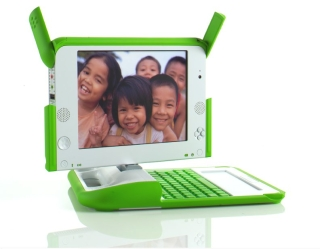
\includegraphics[width=5cm]{files/nigerian-machine.jpg} &
      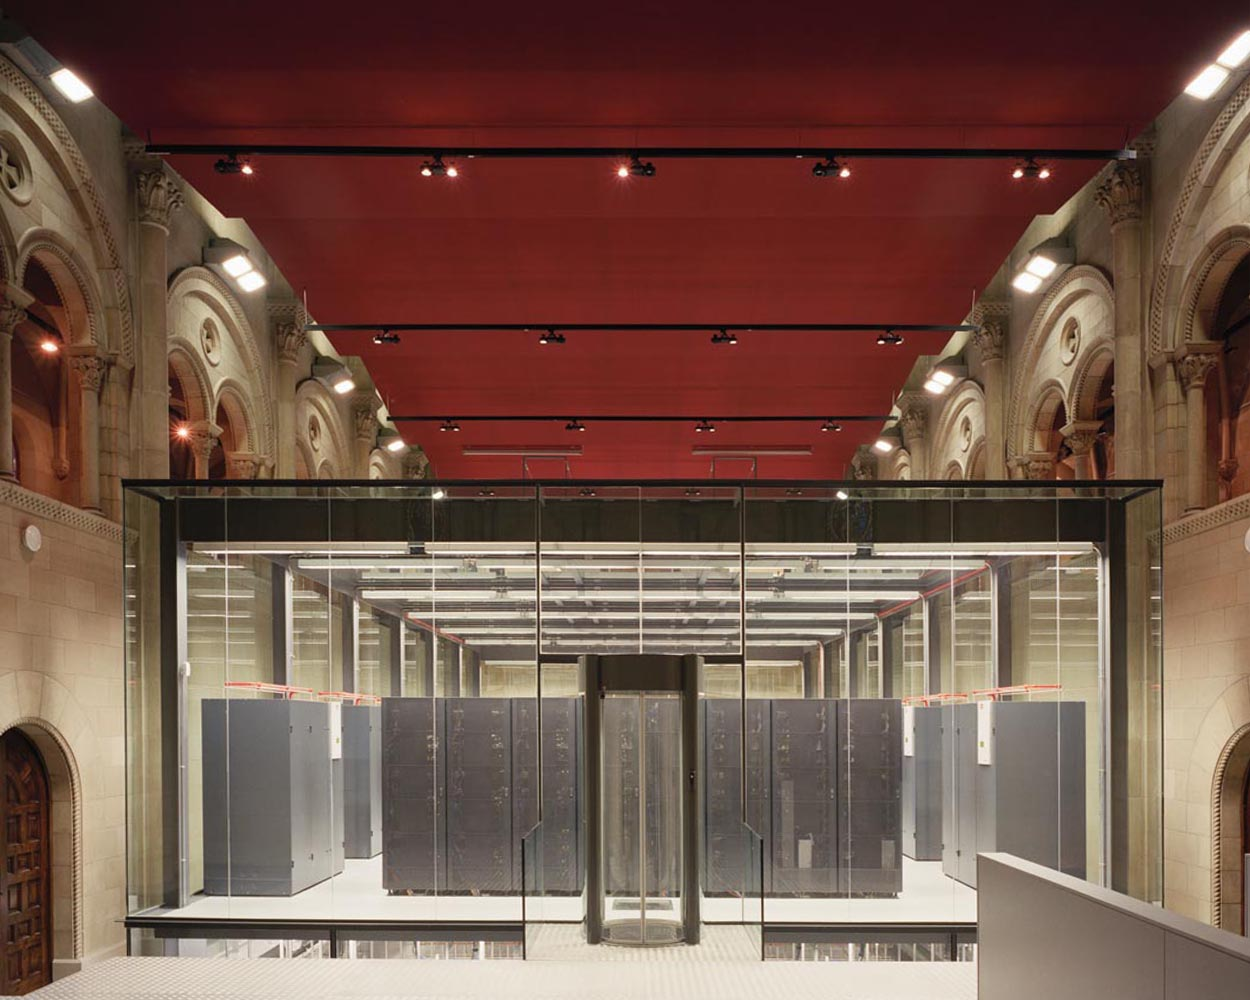
\includegraphics[width=5cm]{files/marenostrum.jpg}\\
      Pequeño & Grande
    \end{tabular}
  \end{center}
\end{frame}

\begin{frame}
  \frametitle{Scripts}
  \begin{itemize}
  \item 1 Procesador
  \item 1 Thread
  \item ejecución $\sim$ segundos
  \item GUI
  \item Normalmente < $10^3$ lineas de código.
  \end{itemize}
\end{frame}

\begin{frame}
  \frametitle{HPC}
  \begin{itemize}
  \item > 8 Procesadores
  \item > 8 Procesos o Threads
  \item ejecución $\sim$ horas
  \item no GUI
  \item Quizás > $10^3$ líneas de código.
  \end{itemize}
\end{frame}

\begin{frame}
  \frametitle{Dos mundos distintos}
  \begin{center}
    \begin{tabular}[h]{cc}
      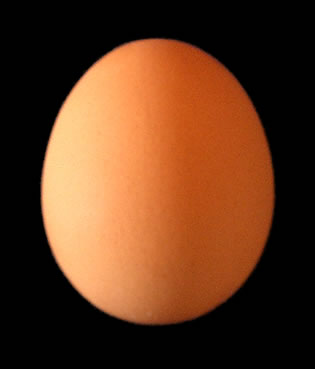
\includegraphics[width=5cm]{files/huevo.jpg} &
      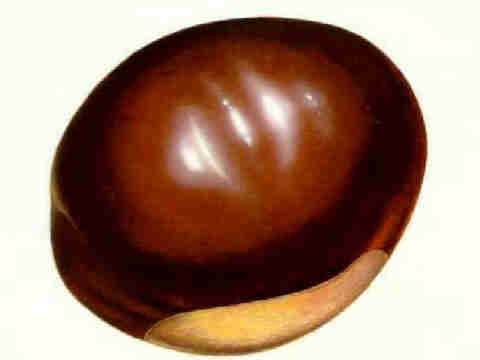
\includegraphics[width=5cm]{files/castana.jpg}\\
      Huevo & Castaña
    \end{tabular}
  \end{center}
\end{frame}


\begin{frame}
  \frametitle{¿Por qué se llama Python?}
  Python debe su nombre a...
\end{frame}

\begin{frame}
  \begin{center}
    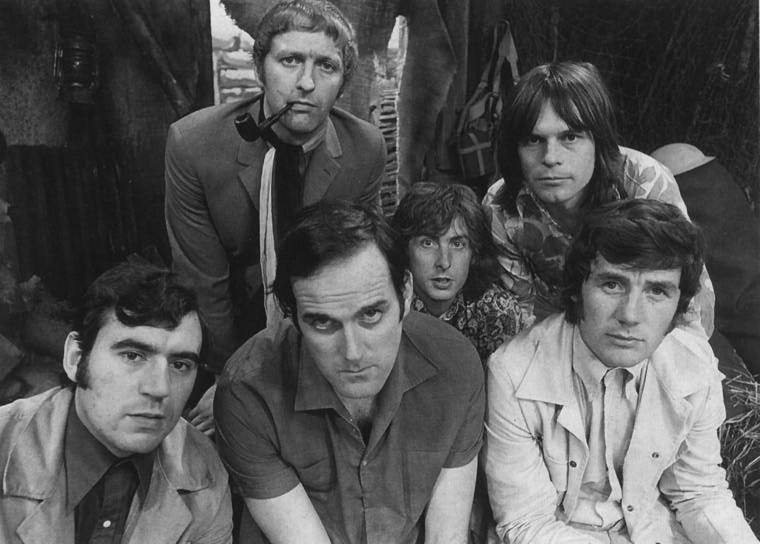
\includegraphics[width=9cm]{files/python.jpg}\\
    % python.jpg: 760x544 pixel, 72dpi, 26.81x19.19 cm, bb=0 0 760 544
    Monty Python
  \end{center}

\end{frame}

\begin{frame}
  \frametitle{¿Quién usa Python?}

  \begin{center}
    
\includegraphics[width=3cm]{files/google.jpg}
    
\includegraphics[width=3cm]{files/Industrial_Light_and_Magic.jpg}
    
\includegraphics[width=3cm]{files/NASA_Logo.jpg}\\
    
\includegraphics[width=3cm]{files/honeywell_logo.jpg}
  \end{center}
\end{frame}

\begin{frame}
  \frametitle{¿Para qué sirve Python?}
  \begin{center}
    Prácticamente para cualquier cosa que se nos pueda ocurrir
  \end{center}

\end{frame}

\begin{frame}
  \frametitle{Desde páginas web...}
  \begin{center}
    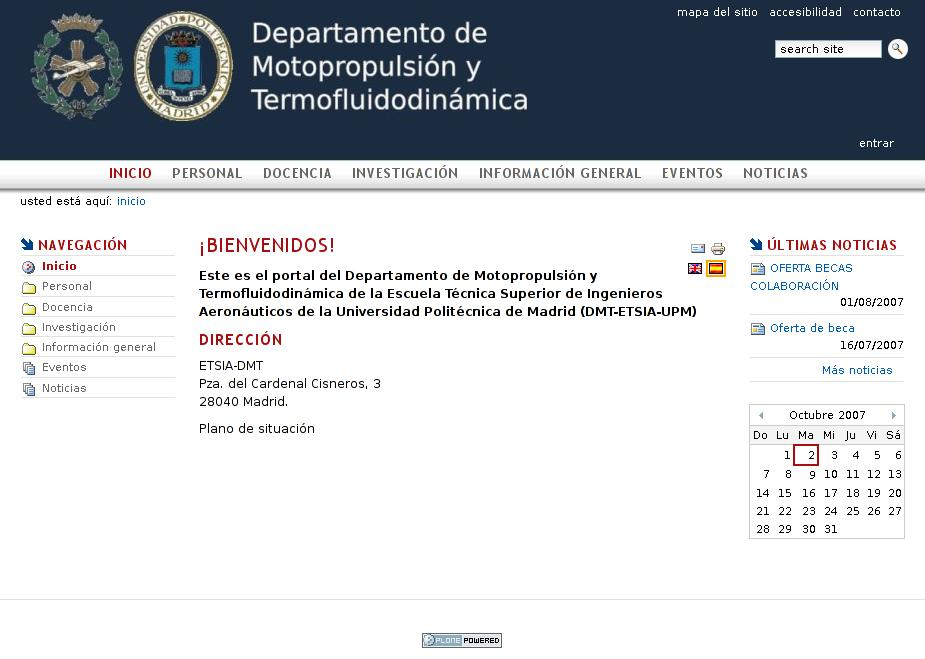
\includegraphics[width=9cm]{files/snapshot1.jpg}\\
    % snapshot1.jpg: 925x659 pixel, 762dpi, 3.08x2.20 cm, bb=0 0 87 62
    Plone, Zope
  \end{center}

\end{frame}

\begin{frame}
  \frametitle{...A utilidades para bioinformática}
  \begin{center}
    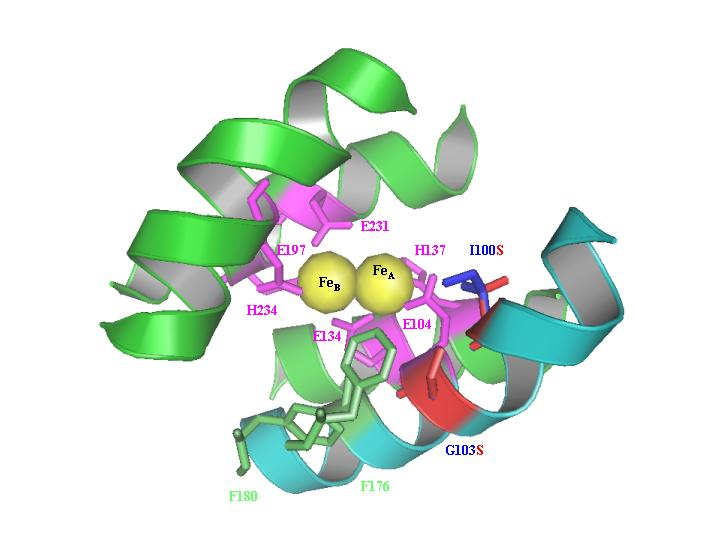
\includegraphics[width=8cm]{files/pymol.jpg}\\
    % pymol.jpg: 720x540 pixel, 72dpi, 25.40x19.05 cm, bb=0 0 720 540
    Pymol
  \end{center}

\end{frame}

\begin{frame}
  \frametitle{Principales características de Python}

  \begin{itemize}
  \item Software Libre (Licencia estilo BSD)
  \item Interpretado
  \item Interactivo
  \item Multiparadigma
    \begin{itemize}
    \item Procedimental
    \item Modular
    \item Orientado a Objetos
    \end{itemize}
  \item Multiplataforma
  \item Especificación especialmente corta (IronPython, Jython, PyPy,
    tinypy ...)
  \item \emph{Incluye las pilas}
  \item ...
  \end{itemize}

\end{frame}

\begin{frame}
  \frametitle{¿Por qué Python se está volviendo tan popular}
  \begin{itemize}
  \item Fácil de aprender
  \item Fácil de ampliar
  \item Consistente por diseño
  \item Impone un buen estilo de programación
  \item Soporta todas las prácticas propuestas por XP, Agile.
  \end{itemize}
  \begin{center}
    Porque es divertido
  \end{center}
\end{frame}

\begin{frame}
  \frametitle{¿Por qué Python y no otro lenguaje?}
  \begin{itemize}
  \item Fácilmente extensible.
    \begin{itemize}
    \item CPython, escrito en ANSI C.
    \end{itemize}
  \item Dinámico.
  \item Software Libre.
  \item Excelente documentación.
  \end{itemize}
\end{frame}


\begin{frame}
  \begin{center}
    \begin{LARGE}
      ¿Qué pinta tiene código escrito en Python?
    \end{LARGE} 
  \end{center}
\end{frame}

\defverbatim[colored]\testcode{
  \begin{lstlisting}
    guillem@aiguaviva ~> python
    Python 2.4.4 (#1, Sep 25 2007, 21:44:53)
    [GCC 4.1.2 (Gentoo 4.1.2)] on linux2
    Type "help", "copyright", "credits" or "license" ...
    >>> import cmath
    >>> i=cmath.sqrt(-1) #Los namespaces son objetos
    >>> i.conjugate() #Los numeros son objetos
    -1j
    >>> i.imag
    1.0
    >>> i.real
    0.0
    >>> i+=3 
    >>> i
    (3+1j)
  \end{lstlisting}
}

\begin{frame}
  \frametitle{Todo es un objeto}
  \testcode
\end{frame}

\defverbatim[colored]\testcode{
  \begin{lstlisting}
    >>> def sumauno(numero):
    ...     return numero+1
    ...
    >>> sumauno(i)
    (4+1j)
  \end{lstlisting}
}
\begin{frame}
  \frametitle{Definir funciones es muy fácil}
  \testcode
  \begin{itemize}
  \item No hay llaves ni ends, los niveles se definen por el sangrado.
  \end{itemize}
\end{frame}


\defverbatim[colored]\testcode{
  \begin{lstlisting}
    >>> def docfunc():
    ...     """Esta es una funcion documentada, a diferencia
    ...     de Matlab la documentacion de las funciones de
    ...     Python es extraible y formateable"""
    ...     pass
    ...
    >>> help(docfunc)
    Help on function docfunc in module __main__:

    docfunc()
    Esta es una funcion documentada, a diferencia de
    Matlab la documentacion de las funciones de Python
    es extraible y formateable
  \end{lstlisting}}

\begin{frame}
  \frametitle{Documentaci\'on a la Matlab}
  \begin{scriptsize}
    \testcode  
  \end{scriptsize}
\end{frame}


%%%%%%%%%%%%%%%% Scripting %%%%%%%%%%%%%%%%%%

\begin{frame}
  \frametitle{python para huevos (pequeños)}
  \begin{center}
    \begin{tabular}[h]{ccc}
      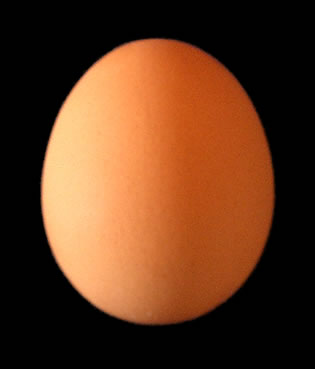
\includegraphics[width=5cm]{files/huevo.jpg} & &
      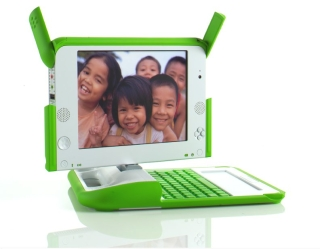
\includegraphics[width=5cm]{files/nigerian-machine.jpg}\\
      Huevo & = &Pequeño
    \end{tabular}
  \end{center}
\end{frame}

\begin{frame}
  \frametitle{Somos insaciables.}
  Queremos un lenguaje de programación...
  \begin{itemize}
  \item Que sea completo según Turing.
  \item Que lo haga \textbf{todo}
  \item Que lo haga \textbf{bien}
  \item Que no me cueste
  \item Que no tenga que mirar el manual
  \item Que ejecute en cualquier sitio.
  \end{itemize}
\end{frame}

\begin{frame}
  \frametitle{¿Java?}
  \begin{itemize}
  \item ¿Matemáticas con Java?
  \item ¿Ganancia respecto a C++?
  \item ¿Existe una comunidad de usuarios?
  \end{itemize}
\end{frame}

\begin{frame}
  \frametitle{Matlab}
  \begin{itemize}
  \item Uno de los lenguajes de programación más patéticos que he
    visto
  \item ¿Por qué pagar $\sim$ 10000 Euros por algo que no lo vale?
  \end{itemize}
\end{frame}

\begin{frame}
  \frametitle{Mathematica, Maple...}
  \begin{center}
    DSL. He dicho lenguaje de programación.
  \end{center}
\end{frame}

\begin{frame}
  \begin{center}
    
\includegraphics[width=9cm]{files/python-logo-generic.pdf}\\
    % python-logo-generic.pdf: 389x115 pixel, 72dpi, 13.72x4.06 cm, bb=0
    % 0 389 115
  \end{center}
  \texttt{import this}
\end{frame}

\defverbatim[colored]\testcode{
  \begin{lstlisting}
    >>> 2+2 #Suma
    4
    >>> 2-1 #Resta
    1
    >>> 2*4.5 #Multiplicacion
    9.0
    >>> 2/4.5 #Division
    0.44444444444444442
  \end{lstlisting}}

\begin{frame}
  \frametitle{Operaciones aritméticas}
  \testcode
  \begin{itemize}
  \item División entera (Python 3.x)
  \item Potencia
  \end{itemize}
\end{frame}

\defverbatim[colored]\testcode{
  \begin{lstlisting}
    >>> import math as m
    >>> import cmath as c
    >>> a=3.0+4.0j
    >>> a/complex(2,1.3)
    (1.968365553602812+0.72056239015817214j)
    >>> c.exp(_)
    (5.3794960137747223+4.7235385533272529j)
    >>> m.exp(abs(_))
    1285.5809221999864
  \end{lstlisting}}

\begin{frame}
  \frametitle{Números complejos y módulos}
  \testcode
\end{frame}


\defverbatim[colored]\testcode{
  \begin{lstlisting}
    >>> import cmath
    >>> help(cmath.acos)
    Help on built-in function acos in module cmath:

    acos(...)
    acos(x)

    Return the arc cosine of x.
  \end{lstlisting}
}
\begin{frame}
  \frametitle{Ayuda}
  \testcode
\end{frame}

\defverbatim[colored]\testcode{
  \begin{lstlisting}
    >>> x = int(raw_input("Por favor, introduzca un entero: "))
    >>> if x < 0:
    ...      x = 0
    ...      print 'Era negativo y lo he cambiado a cero'
    ... elif x == 0:
    ...      print 'Cero'
    ... elif x == 1:
    ...      print 'Uno'
    ... else:
    ...      print 'Mas'
    ...
  \end{lstlisting}
}
\begin{frame}
  \frametitle{If}
  \testcode
\end{frame}

\defverbatim[colored]\testcode{
  \begin{lstlisting}
    >>> a = ['gato', 'ventana', 'defenestrar']
    >>> for x in a:
    ...     print x, len(x)
    ... 
    gato 4
    ventana 7
    defenestrar 11
    >>> for x in a: # Haced esto y morid
    ...    if len(x) > 6: a.insert(0, x)
  \end{lstlisting}
}
\begin{frame}
  \frametitle{for}
  ¡\textbf{Es un iterador}!
  \testcode
\end{frame}

\defverbatim[colored]\testcode{
  \begin{lstlisting}
    >>> range(4)
    [0, 1, 2, 3]
    >>> range(3,12,3)
    [3, 6, 9]
  \end{lstlisting}
}
\begin{frame}
  \frametitle{range}
  \testcode
\end{frame}


\defverbatim[colored]\testcode{
  \begin{lstlisting}
    def fib2(n): 
    """Devuelve una lista con la serie de 
    Fibonacci hasta n."""
    result = []
    (a, b) = (0, 1)
    while b < n:
    result.append(b)
    (a, b) = (b, a+b)
    return result
  \end{lstlisting}
}
\begin{frame}
  \frametitle{Definición de funciones}
  \testcode
\end{frame}


\defverbatim[colored]\testcode{
  \begin{lstlisting}
    >>> def make_incrementor(n):
    ...     return lambda x: x + n
    ...
    >>> f = make_incrementor(42)
    >>> f(0)
    42
    >>> f(1)
    43
  \end{lstlisting}
}
\begin{frame}
  \frametitle{Funciones Lambda}
  \testcode
\end{frame}


\begin{frame}
  \frametitle{Tipos}
  \begin{itemize}
  \item Enteros
  \item Números en coma flotante
  \item Números complejos
  \item Cadenas de texto
  \item Listas
  \item Tuples
  \item Conjuntos
  \item Diccionarios
  \end{itemize}
\end{frame}

\defverbatim[colored]\testcode{
  \begin{lstlisting}
    a.__add__           a.__iadd__          a.__rmul__
    a.__class__         a.__imul__          a.__setattr__
    a.__contains__      a.__init__          a.__setitem__
    a.__delattr__       a.__iter__          a.__setslice__
    a.__delitem__       a.__le__            a.__str__
    a.__delslice__      a.__len__           a.append
    a.__doc__           a.__lt__            a.count
    a.__eq__            a.__mul__           a.extend
    a.__ge__            a.__ne__            a.index
    a.__getattribute__  a.__new__           a.insert
    a.__getitem__       a.__reduce__        a.pop
    a.__getslice__      a.__reduce_ex__     a.remove
    a.__gt__            a.__repr__          a.reverse
    a.__hash__          a.__reversed__      a.sort
  \end{lstlisting}
}
\begin{frame}
  \frametitle{Listas}
  \begin{scriptsize}
    \testcode
  \end{scriptsize}
\end{frame}

\defverbatim[colored]\testcode{
  \begin{lstlisting}
    >>> [(x, x**2) for x in vec]
    [(2, 4), (4, 16), (6, 36)]
    >>> vec1 = [2, 4, 6]
    >>> vec2 = [4, 3, -9]
    >>> [x*y for x in vec1 for y in vec2]
    [8, 6, -18, 16, 12, -36, 24, 18, -54]
    >>> [x+y for x in vec1 for y in vec2]
    [6, 5, -7, 8, 7, -5, 10, 9, -3]
    >>> [vec1[i]*vec2[i] for i in range(len(vec1))]
    [8, 12, -54]
  \end{lstlisting}
}
\begin{frame}
  \frametitle{List comprehensions}
  \testcode
\end{frame}

\begin{frame}
  \frametitle{Ejercicio}
  Crear una lista que contenga las cadenas de texto\texttt{uno},
  \texttt{dos}, \texttt{tres} y \texttt{cuatro}.  Mover los elementos
  que contienen la letra \emph{o} a una lista nueva. Primero hacerlo
  con un bucle y luego mediante un \emph{list comprehension} (en una
  línea).
\end{frame}

\begin{frame}
  \frametitle{La biblioteca estándar}
  \begin{itemize}
  \item Manipulación textual
  \item Envío de correos electrónicos
  \item Proceso de contenido en XML, csv, XDR...
  \item Criptografía
  \item Interacción con el sistema operativo
  \item Compresión de datos
  \item Almacenamiento de variables
  \item Enlazado con librerías externas.
  \item Acceso a las funcionalidades POSIX
  \end{itemize}
\end{frame}

\begin{frame}
  \frametitle{La biblioteca estándar II}
  \begin{itemize}
  \item IPC y redes.
  \item Protocolos de internet (XMLRPC, cookies, cgi, smtp, http, ftp...)
  \item Multimedia
  \item GUI
  \item Internacionalización
  \item Documentación
  \item Tests
  \item Debugging
  \item Profiling
  \end{itemize}
\end{frame}

\begin{frame}
  \frametitle{Ejercicio}
  A partir del módulo os ejecutar la orden \texttt{ls} para ver el
  contenido del directorio actual.
\end{frame}

\begin{frame}
  \frametitle{Ejercicio}
  A partir del módulo sys conseguir que un programa escrito en Python
  devuelva una ayuda al pasarle el argumento \emph{-h}
\end{frame}


%%%%%%%%%%%%%% Objetos %%%%%%%%%%%%%%%%

\begin{frame}
  \frametitle{Orientación a objetos}
  \begin{itemize}
  \item Paradigma de implementación de algoritmos
  \item Pretende adaptarse a la realidad
  \item Estructura que puede contener datos y métodos
  \item Los objetos pueden relacionarse entre ellos mediante la
    herencia
  \item El método más común es generar una instancia a partir de una
    clase
  \end{itemize}
\end{frame}

\defverbatim[colored]\testcode{
\begin{lstlisting}
In [1]: import math as m

In [2]: class Complex(object):
   ...:     def __init__(self, realp, imagp):
   ...:         self.r = realp
   ...:         self.i = imagp
   ...:
   ...:     def abs(self):
   ...:         return m.sqrt(self.r**2+self.i**2)
   ...:
\end{lstlisting} 
}
\begin{frame}
  \frametitle{Orientación a objetos}
  \testcode
\end{frame}

\defverbatim[colored]\testcode{
\begin{lstlisting}
In [3]: nc = Complex(3,4)#instancia de clase

In [4]: nc.r
Out[4]: 3

In [5]: nc.i
Out[5]: 4

In [6]: nc.abs()
Out[6]: 5.0
\end{lstlisting} 
}
\begin{frame}
  \frametitle{Orientación a objetos}
  \testcode
\end{frame}

\begin{frame}
  \frametitle{Herencia}
  \begin{itemize}
  \item El mecanismo de extensión es la herencia
  \item Sirve para crear una \emph{jerarquía} de objetos
  \item Si una clase cede su contenido se llama clase \emph{padre} o
    \emph{parent}
  \item La clase que se genera a partir de la \emph{parent} es la
    clase \emph{hijo}
  \item Una clase puede heredar de varias clases superiores.
  \end{itemize}
\end{frame}


\defverbatim[colored]\testcode{
\begin{lstlisting}
class MoreComplex(Complex):
    def __init__(self, realp, imagp):
        Complex.__init__(self,realp,imagp)

    def arg(self):
        return m.atan(self.i/self.r)

In [14]: mc = MoreComplex(3,4)

In [15]: mc.arg()
Out[15]: 0.78539816339744828
\end{lstlisting} 
}
\begin{frame}
  \frametitle{Herencia}
  \testcode
\end{frame}


\defverbatim[colored]\testcode{
\begin{lstlisting}
 >>> class pato:
...     cantidad = 1
...     def haz_cua(self):
...           print "cua!"
...
...     def reproducete(self):
...           cantidad += 1
...
>>> estoesunpato=pato() #instancia de pato
>>> estoesunpato.cantidad
1
>>> estoesunpato.haz_cua()
cua!
\end{lstlisting} 
}

\begin{frame}
\frametitle{Duck typing}
\testcode
\end{frame}

\defverbatim[colored]\testcode{
\begin{lstlisting}
>>> estoesunpato=pato() #instancia de pato
>>> cuaqueador(estoesunpato)
cua!
>>> class guillem:
...     def haz_cua(self):
...             print "cua!"
...
>>> falsopato=guillem() #ese soy yo
>>> cuaqueador(falsopato)
cua!
>>> isinstance(falsopato,pato)
False
\end{lstlisting}
}
\begin{frame}
\frametitle{Duck typing}
\testcode

Si algo anda como un pato y hace cua como un pato para mi va a ser un pato.
Para la función cuaqueador yo soy tan pato como un pato.
\end{frame}

%%%%%%%%%%% NumPy y SciPy %%%%%%%%%%%%%

\begin{frame}
  \frametitle{Numpy}

  \begin{itemize}
  \item Proporciona a Puython el tipo \texttt{array}
  \item Un \texttt{array} es un tipo:
    \begin{itemize}
    \item Homogéneo en memoria
    \item Definido por sus dimensiones y el tipo de sus datos.
    \item Pensado para operaciones vectoriales.
    \end{itemize}
  \item Funciones matemáticas básicas
  \end{itemize}
\end{frame}

\defverbatim[colored]\testcode{
\begin{lstlisting}
>>> from numpy import array
>>> help(array)

Help on built-in function array in module numpy.core.multiarray:

array(...)
    array(object, dtype=None, copy=1,order=None, subok=0,ndmin=0)

    Return an array from object with the specified date-type.

    Inputs:
      object - an array, any object exposing the array interface, any
                object whose __array__ method returns an array, or any
                (nested) sequence.
      dtype  - The desired data-type for the array.  If not given,
                then the type will be determined as the minimum type
                required
   [...]
\end{lstlisting}
}
\begin{frame}
  \frametitle{El tipo \texttt{array}}
  \testcode
\end{frame}

\begin{frame}
  \frametitle{Creación}
  \begin{itemize}
  \item A la Matlab
    \begin{itemize}
    \item \texttt{zeros}
    \item \texttt{ones}
    \item \texttt{linspace}
    \end{itemize}
  \item A la Python
    \begin{itemize}
    \item \texttt{array}
    \item \texttt{empty}
    \item \texttt{arange}
    \end{itemize}
  \end{itemize}
\end{frame}

\begin{frame}
  \frametitle{slicing}
\end{frame}

\begin{frame}
  \frametitle{Métodos}
\end{frame}

\begin{frame}
  \texttt{Ufuncs}
\end{frame}

\begin{frame}
  \frametitle{Almacenamiento}
\end{frame}

\begin{frame}
  \frametitle{Scipy}
\end{frame}


\begin{frame}
  \frametitle{Sage}
  
\end{frame}
%%%%%%%%%%%%%%%% HPC %%%%%%%%%%%%%%%%%%


\begin{frame}
 \frametitle{python para castañas (grandes)}
  \begin{center}
 \begin{tabular}[h]{ccc}
   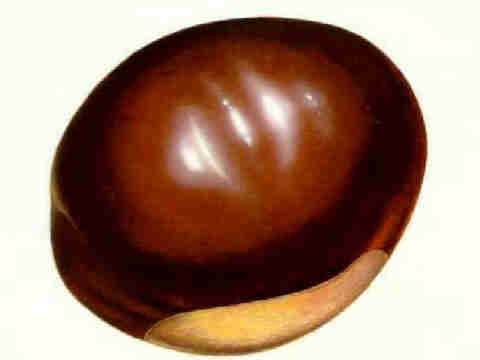
\includegraphics[width=5cm]{files/castana.jpg}& &
   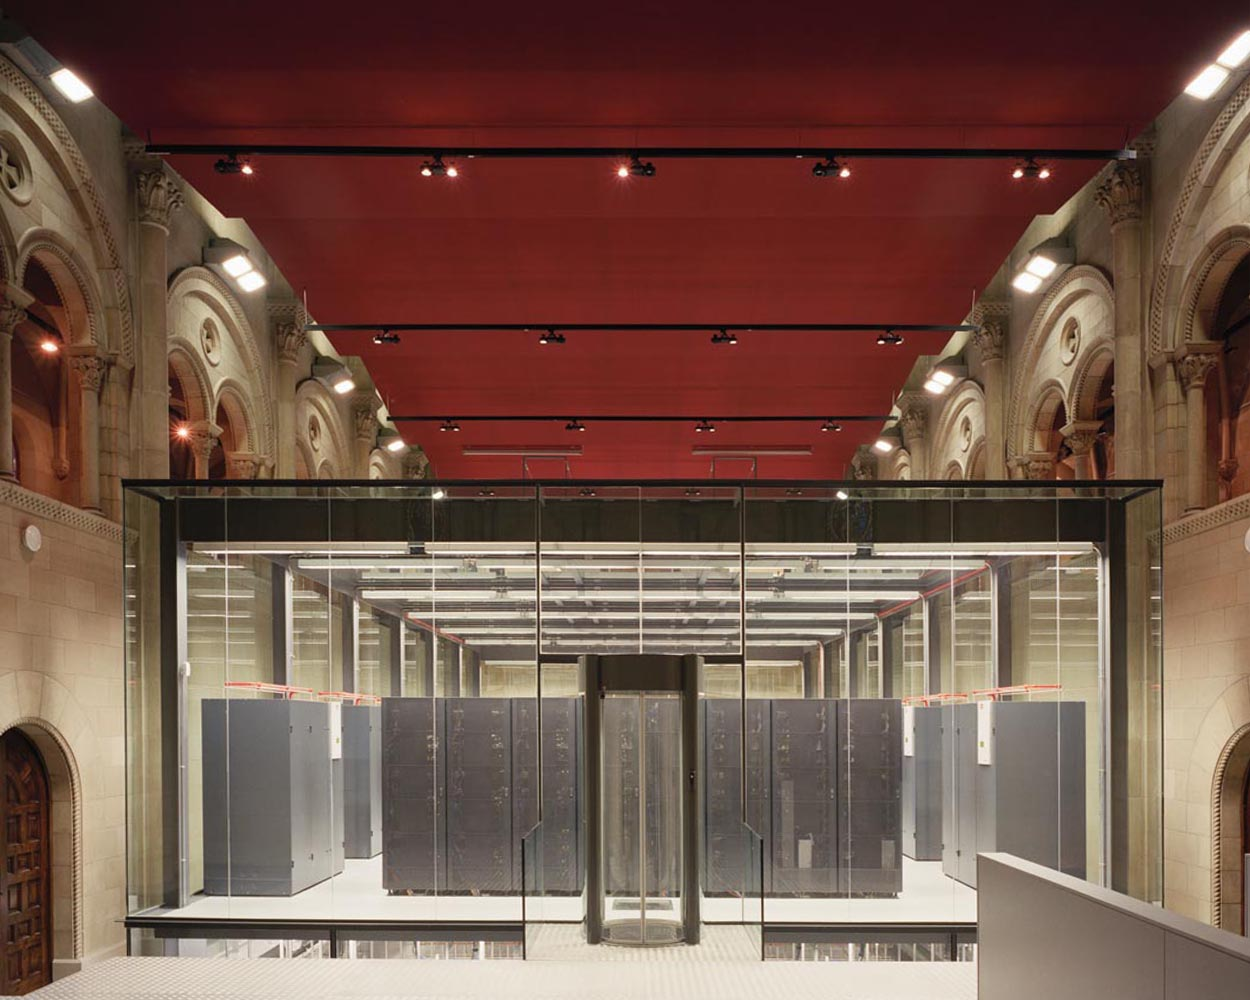
\includegraphics[width=5cm]{files/marenostrum.jpg}\\
   Castaña & = & Grande
 \end{tabular}
\end{center}
\end{frame}

\begin{frame}
  \frametitle{Same old story}
  \begin{center}
    \begin{Huge}
      \textbf{HPC = Fortran, C}
    \end{Huge}
  \end{center}
\end{frame}

\begin{frame}
  \frametitle{Ganaremos}
  \begin{itemize}
  \item Velocidad
  \item Gestión directa de la memoria
  \item ¿Algo más?
  \end{itemize}
\end{frame}

\begin{frame}
  \frametitle{Perderemos:}
  \begin{itemize}
  \item Interactividad
  \item Garbage collection
  \item Versatilidad
  \item Sencillez
  \item Librerías
  \end{itemize}
\end{frame}

\begin{frame}
  \begin{center}
    \begin{LARGE}
    ¿Podemos quedarnos con lo mejor de los dos mundos?      
    \end{LARGE}
  \end{center}
\end{frame}

\begin{frame}
  \frametitle{¿Por qué los lenguajes interpretados son lentos?}
  Porque son dinámicos.
  \begin{center}
    \begin{tikzpicture}      
      \node (lexer) at (0,0) [draw=black, thick, fill=black!10]
      {Lexer};

      \node (parser) at (2,0) [draw=black, thick, fill=black!10]
      {Parser};

      \node (encoder) at (4,0) [draw=black, thick, fill=black!10]
      {Encoder};

      \node (vm) at (7,0) [draw=black, very thick, fill=black!10]
      {VM};

      \node (codigo) at (0,1) [draw=blue,rounded
      corners,thick,fill=blue!20] {Codigo};

      \node (tokens) at (1,-1) [draw=blue,rounded
      corners,thick,fill=blue!20]
      {Tokens};

      \node (tokensp) at (3,1) [draw=blue,rounded
      corners,thick,fill=blue!20]
      {Tree};

      \node (bytecode) at (5.5,-1) [draw=blue,rounded
      corners,thick,fill=blue!20]
      {Bytecode};

      \node (assembler) at (8.5,1) [draw=blue,rounded
      corners,thick,fill=blue!20]
      {Assembler};
      
      \draw[->] (codigo.south) -- (lexer.north);

      \draw[->] (lexer.south) |- (tokens.west);

      \draw[->] (tokens.east) -| (parser.south);

      \draw[->] (parser.north) |- (tokensp.west);

      \draw[->] (tokensp.east) -| (encoder.north);

      \draw[->] (encoder.south) |- (bytecode.west);

      \draw[->] (bytecode.east) -| (vm.south);
      
      \draw[->] (vm.north) |- (assembler.west);
    \end{tikzpicture}
  \end{center}

\end{frame}

\begin{frame}
  \frametitle{Lenguajes dinámicos}
  \begin{itemize}
  \item El tipo de las variables sólo se sabe en tiempo de ejecución.
  \item El bytecode mueve un \textit{objectspace} o \textit{stack}
  \item El ensamblador de la máquina virtual hace lo que le dice el
    bytecode.
  \item La máquina virtual es incapaz de generar ensamblador
    optimizado.
  \item Dos planteamientos para lenguajes dinámicos
    \begin{itemize}
    \item Duck typing
    \item Type inference
    \end{itemize}
  \end{itemize}
\end{frame}

\begin{frame}
  \frametitle{Type inference}
  \begin{itemize}
  \item Intenta descubrir los tipos de cada variable en tiempo de
    compilación.
  \item El lenguaje es dinámico en apariencia pero estático en
    memoria.
  \item Menos dinámico que el Duck typing.
    \begin{itemize}
    \item Errores en tiempo de compilación
    \item Casting automático.
    \end{itemize}
  \item Mejor rendimiento.
  \end{itemize}
\end{frame}

\begin{frame}
  \frametitle{JIT}
  Just In Time
  \begin{itemize}
  \item Método para optimizar el bytecode.
    \begin{itemize}
    \item Analiza el bytecode.
    \item Hace type inference.
    \item Genera ensamblador optimizado para la arquitectura.
    \end{itemize}
  \item Matlab lo utiliza para los bucles.
  \item Octave va detrás de ello.
  \item Python no tiene... PyPy sí, aunque muy verde.
  \end{itemize}
\end{frame}

\begin{frame}
  \frametitle{Global Interpreter Lock}
  Otro problema de python (y otros).
  \begin{itemize}
  \item La máquina virtual sólo puede ejecutar un thread.
  \item No tendremos multithreading por muy trivial que quede en el
    bytecode.
  \item Si queremos threads tendremos que pedirlos
  \item Estensiones con propia gestión de threads.
  \item Con un poco de suerte se arreglará, de otra forma python
    morirá.
  \end{itemize}
\end{frame}

\begin{frame}
  \frametitle{La solución}
  \begin{center}
    \begin{Huge}
      Optimización Selectiva
    \end{Huge}
  \end{center}
  \vspace{1cm}
  \begin{flushright}
    \textit{We should forget about small efficiencies, say about 97\%
      of the time: premature optimization is the root of all evil. Yet
      we should not pass up our opportunities in that critical 3\%}. Knuth
  \end{flushright}
\end{frame}

\begin{frame}
  \frametitle{La regla del 80-20}
  \begin{itemize}
  \item El 80\% del código se escribe en el 20\% de tiempo.
  \item El 80\% del código es para tareas triviales, sólo el 20\%
    calcula algo de verdad.
  \item Del anterior, sólo el 20\% es realmente intensivo.
  \item Ergo sólo tendremos que optimizar un 5\% del código.
  \end{itemize}
\end{frame}

\begin{frame}
  \frametitle{Estrategia a seguir}
  \begin{flushright}
    \textit{Bottlenecks occur in surprising places, so don't try to
      second guess and put in a speed hack until yo have proven that's
      where the bottleneck is}. Rob Pike
  \end{flushright}
  \vspace{1cm}
  \begin{itemize}
  \item Hacer un buen profiling del código.
  \item Descubrir los cuellos de botella.
  \item \textbf{Eliminar el componente dinámico del lenguaje donde sea
    estrictamente necesario.}
  \end{itemize}
\end{frame}

\begin{frame}
  \begin{center}
    \begin{Huge}
      Siempre que no tengamos que paralelizar.
    \end{Huge}
  \end{center}
\end{frame}


\begin{frame}
  \frametitle{Para ello...}
  \begin{itemize}
  \item Escribir extensiones a la Máquina virtual con C (Python.h)
  \item Escribir módulos en Fortran (f2py)
  \item Enlazar al intérprete bibliotecas en C o Fortran (ctypes,
    swig)
  \item Utilizar un lenguaje de extensión (pyrex, cython)
  \item Crear nuestra propia versión de python (PyPy)
  \item[$\rightarrow$] Utilizar un intérprete preparado para el cálculo paralelo
    (ipython1)
  \end{itemize}
\end{frame}

\begin{frame}
\begin{center}
 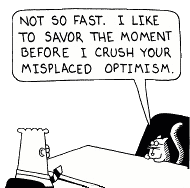
\includegraphics[width=6cm]{files/catbert.png}\\
\end{center}
\end{frame}

\beamertemplatesolidbackgroundcolor{red}

\begin{frame}
  \begin{center}
    \begin{Huge}
      \color{white}{\textbf{¿Con cuál me quedo?}}
    \end{Huge}
  \end{center}
\end{frame}

\beamertemplatesolidbackgroundcolor{white}

\defverbatim[colored]\testcode{
\begin{lstlisting}
$ python -m profile main.py
         101006 function calls (96090 primitive calls) in 1.740 CPU seconds

   Ordered by: standard name

   ncalls  tottime  percall  cumtime  percall filename:lineno(function)
        1    0.000    0.000    0.000    0.000 :0(__import__)
        2    0.000    0.000    0.000    0.000 :0(__new__)
       15    0.000    0.000    0.000    0.000 :0(_getframe)
      589    0.000    0.000    0.000    0.000 :0(abs)
       38    0.000    0.000    0.000    0.000 :0(acquire_lock)
      144    0.000    0.000    0.000    0.000 :0(add_docstring)
        2    0.000    0.000    0.000    0.000 :0(allocate_lock)
\end{lstlisting}
}
\begin{frame}
  \frametitle{Profiling}
 \testcode 
\end{frame}

\begin{frame}
  \frametitle{Pyrex}
  \begin{itemize}
  \item Lenguaje para escribir extensiones en python
  \item Menos dinámico que Python
  \item Un compilador lo traduce a C y genera el módulo que luego
    enlaza a CPython
  \item El proceso de creación del módulo es lento pero una vez se ha
    enlazado conseguimos velocidades parecidas a las de C.
  \end{itemize}
\end{frame}

\begin{frame}
  \frametitle{f2py}
  \begin{center}
    Una oportunidad de utilizar el lenguaje de programación del
    futuro, Fortran.
  \end{center}
\end{frame}

\defverbatim[colored]\testcode{
\begin{lstlisting}
from ctypes import c_int, POINTER #1
import numpy as np
from numpy.ctypeslib import load_library,ndpointer #1

def dgesv(N,A,B):
    A = np.asfortranarray(A.astype(np.float64)) #2
    B = np.asfortranarray(B.astype(np.float64))

    cN=c_int(N)
    NRHS=c_int(1)
    LDA=c_int(N)
    IPIV=(c_int * N)()
    LDB=c_int(N)
    INFO=c_int(1)

    lapack=load_library('liblapack.so','/usr/lib/')#3
\end{lstlisting}
}
\begin{frame}
  \frametitle{ctypes}
  \testcode
\end{frame}


\defverbatim[colored]\testcode{
\begin{lstlisting}
     lapack.dgesv_.argtypes=[POINTER(c_int),
             POINTER(c_int),
             ndpointer(dtype=np.float64,
             ndim=2,
             flags='FORTRAN'),
             POINTER(c_int), POINTER(c_int),
             ndpointer(dtype=np.float64,
                       ndim=2,
                       flags='FORTRAN'),
             POINTER(c_int),POINTER(c_int)]#4

    lapack.dgesv_(cN,NRHS,A,LDA,IPIV,B,LDB,INFO)#5
    return B

print dgesv(2,np.array([[1,2],[1,4]]),np.array([[1,3]]))
\end{lstlisting}
}
\begin{frame}
  \testcode
\end{frame}

\begin{frame}
  \frametitle{PyPy}
  \begin{center}
    La revolución de la abstracción.
  \end{center}
\end{frame}

\end{document}
